\begin{figure}[t]
    \centering
    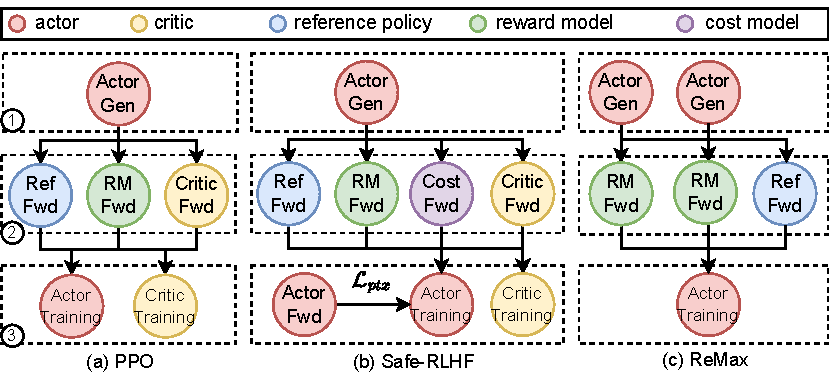
\includegraphics[width=\linewidth]{figs/fig_dataflow_2.pdf}
    \vspace{-6.6mm}
    \caption{Dataflow graph of 3 RLHF algorithms \cite{ouyang2022training, daiSafeRLHFSafe2023, li2023remax}. 
    Stage $\textcircled{1}$, $\textcircled{2}$,  $\textcircled{3}$
    represent Generation, Preparation, and Training, respectively.
    }
    \vspace{-2.4mm}
    \label{fig:rlhf_dataflow}
\end{figure}

\section{Background and Motivation} \label{sec:2_bckground_and_motivation}


\subsection{Reinforcement Learning from Human Feedback} \label{sec:2_1_bckgroud_rlhf}
\noindent\textbf{RLHF Workflow.}
RLHF %
aligns the linguistic space of %
LLMs with human values, using a set of human-ranked candidates of given prompts~\cite{ouyang2022training, bai2022training, daiSafeRLHFSafe2023, shao2024deepseekmath, li2023remax, zheng2023improving, lee2023rlaif}.
An RLHF system typically consists of multiple models, e.g., an actor, a critic, a reference policy, and one or multiple
reward models. The actor and the reference are each pre-trained/fined-tuned LLM (i.e., the LLM that is undergoing RLHF). The critic and reward models can be different LLMs fine-tuned on the human preference dataset, with the language
modeling head replaced by a scalar output head~\cite{ouyang2022training, bai2022training}.
The RLHF workflow can be decomposed into 3 stages (Figure~\ref{fig:rlhf_dataflow}) and we take PPO as an example:

\noindent $\bullet$\textit{Stage 1 (Generation):} The actor produces responses from a batch of prompts using auto-regressive generation.

\noindent $\bullet$\textit{Stage 2 (Preparation): }Using prompts and generated responses, the critic computes their values~\cite{schulman2017proximal, schulman2015trust}, the reference policy computes their reference log probabilities, and the reward model computes their rewards~\cite{ouyang2022training, bai2022training}, all via a single pass of forward computation of the respective model. %

\noindent $\bullet$\textit{Stage 3 (Learning/Training): }The actor and the critic are updated via Adam~\cite{kingma2017adam}, 
using the batch of data produced by previous stages and the loss function~\cite{ouyang2022training}.

Other RLHF algorithms  %
largely follow the 3-stage workflow as well (Figure~\ref{fig:rlhf_dataflow}(b)(c)).
Safe-RLHF~\cite{daiSafeRLHFSafe2023} introduces an auxiliary pretrain loss following PPO-ptx~\cite{ouyang2022training} %
and includes an additional cost model to fit human preferences and safety labels simultaneously. 
ReMax~\cite{li2023remax} %
requires an additional generation pass for variance reduction and eliminates the critic model in the dataflow.
Researchers are actively exploring novel RLHF algorithms~\cite{shao2024deepseekmath, lee2023rlaif, zheng2023improving} and integrating traditional RL methods into RLHF domains~\cite{kaufmann2023survey}. These variances necessitate a flexible representation of the RLHF dataflow graph to accommodate diverse algorithmic requirements.











\begin{figure}[!t]
    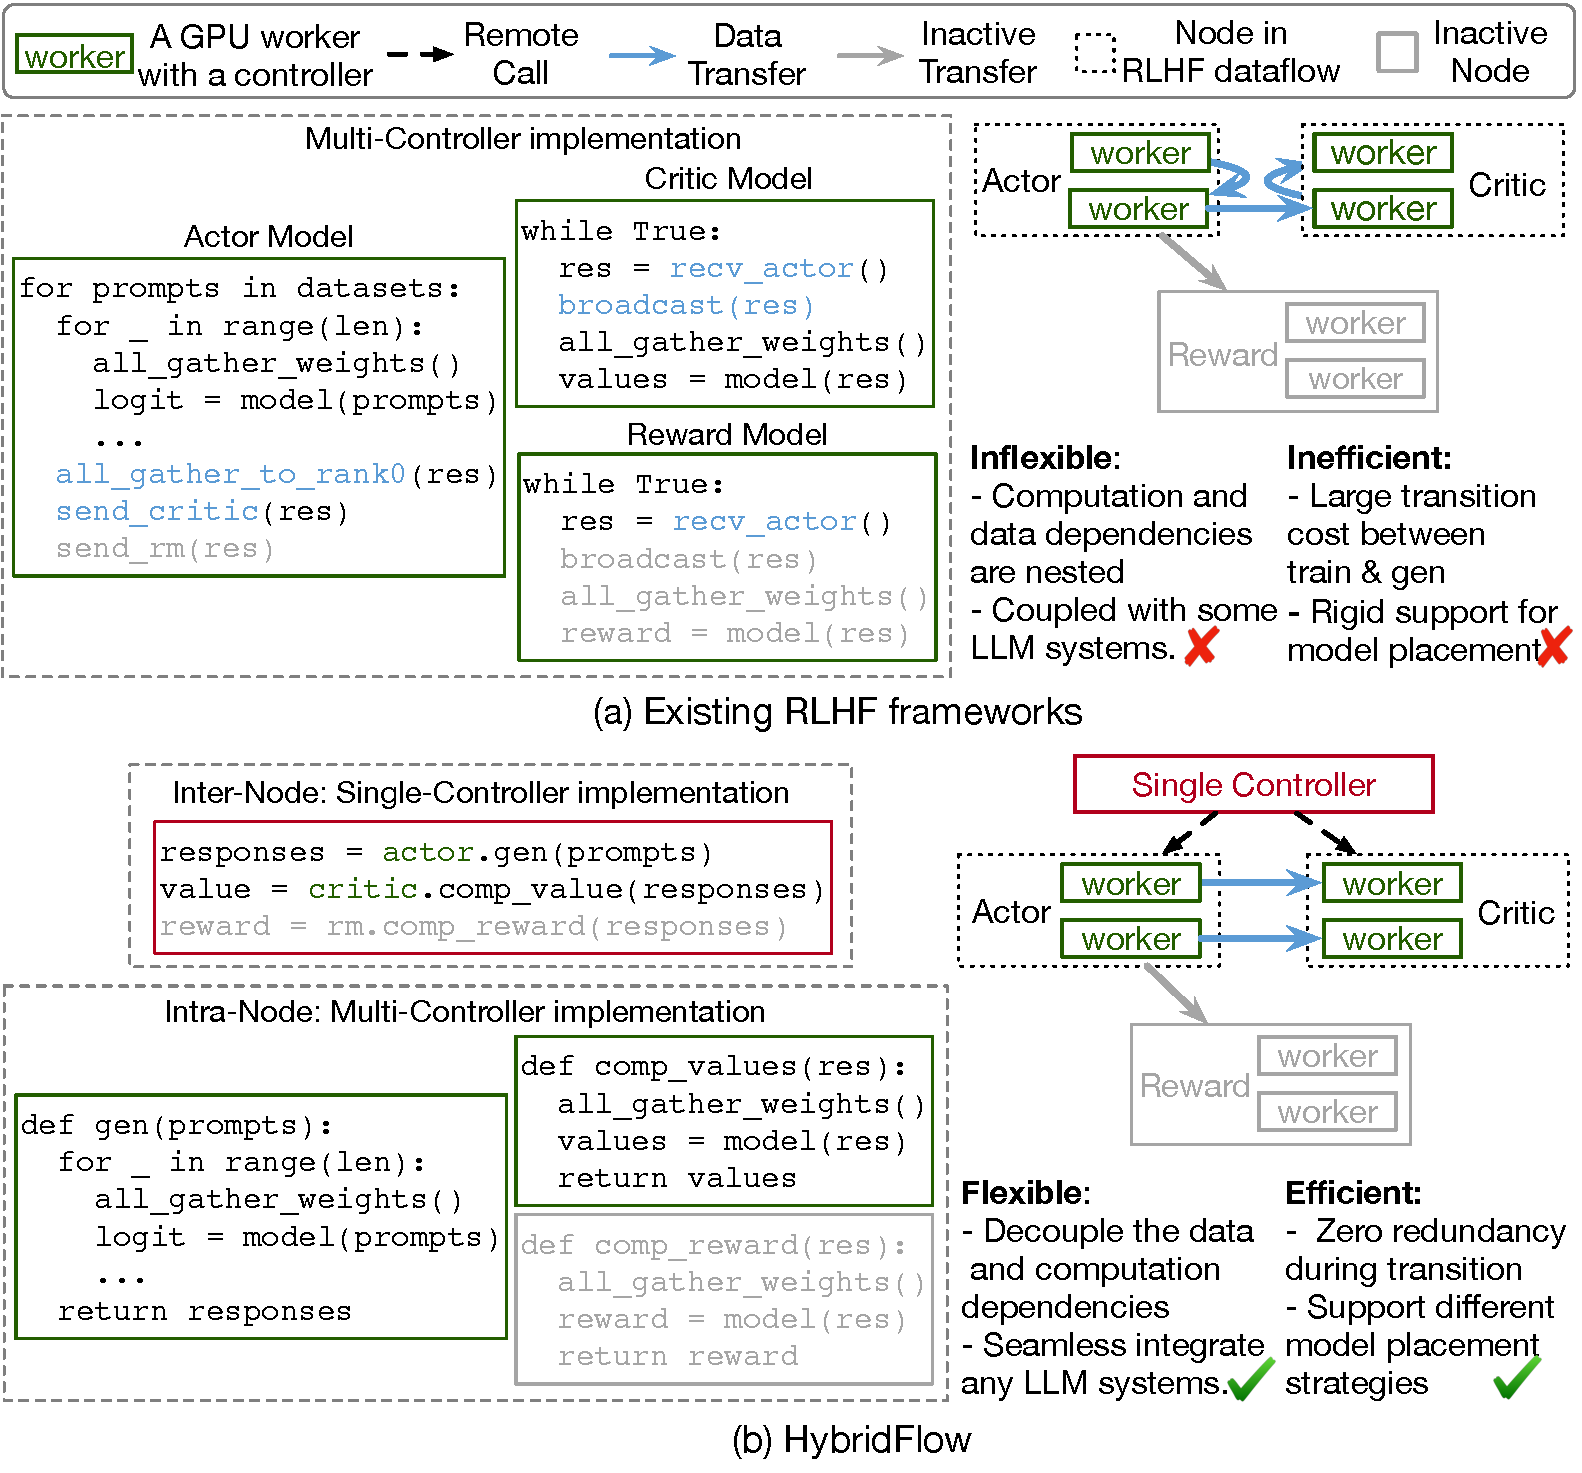
\includegraphics[width=\linewidth]{figs/fig_programming_rlhf_withcode_test.pdf}
    \vspace{-5mm}
    \caption{
    Programming model used in RLHF systems. (a) Existing RLHF systems adopt the \textit{multi-controller} paradigm.
    (b) \sysname{} utilizes a hybrid programming model: the \textit{single-controller} coordinates models; each model uses \textit{multi-controller} paradigm in distributed computation. Inactive node in grey represents operation not executed at this time. 
    }
    \label{fig:program_model_compare}
    \vspace{-3mm}
\end{figure}

\noindent\textbf{Parallelism Strategies.}
LLMs are trained and served with data, pipeline, and tensor parallelism~\cite{narayanan2021efficient,jiang2024megascale, kwon2023efficient}. 
With data parallelism (DP), the input data is split into multiple subsets; each subset is processed %
by a separate %
device (e.g., a GPU)~\cite{sergeev2018horovod}. 
ZeRO~\cite{rajbhandari2020zero} is a memory-optimized solution for DP training, progressively sharding optimizer states, gradients, and model parameters across GPUs.
Pipeline parallelism (PP)~\cite{huang2019gpipe, narayanan2019pipedream} and tensor parallelism (TP)~\cite{shoeybi2019megatron}
distribute model parameters, gradients and optimizer states across multiple GPUs. 
Modern distributed training frameworks like Megatron-LM~\cite{shoeybi2019megatron} and MegaScale~\cite{jiang2024megascale} utilize \textit{3D parallelism} or \textit{PTD parallelism} %
~\cite{narayanan2021efficient}, where P, T, D stand for PP, TP, DP, respectively. %
In 3D parallelism, PP size represents the number of pipeline stages in model training, TP size refers to the number of shards that a tensor is partitioned into, and DP size is the number of model replicas.
LLM serving systems
employ 3D parallelism similar to training while only model parameters and KVCache are sharded~\cite{kwon2023efficient, nvidiaTensorRTLLM, holmes2024deepspeed}. 




LLM models in the RLHF dataflow may %
perform distinct computations, including training (one forward pass, one backward pass and model update), inference (one forward pass) and generation (auto-regressive generation with multiple forward passes). In particular, training and generation are performed on the actor model, training and inference on the critic, and inference on reference policy and reward models.
Distinct parallel strategies can be applied to different models for varied computations to achieve optimal throughput. %


















\subsection{Programming Model for Distributed ML} \label{sec:motivate_programming_model}


\noindent \textbf{Single-Controller.} %
It employs a centralized controller to manage the overall execution flow of the distributed program. With centralized control logic, users can build core functionalities of the dataflow as a single process (Figure~\ref{fig:program_model_compare}(b)), while the controller automatically generates distributed workers to carry out the computation.
With a global view of the hardware and dataflow graph, the single-controller paradigm allows flexible and optimized %
resource mapping and execution order coordination among dataflow tasks. 
However, coordination messages are passed from the controller to all workers, %
incurring significant dispatch overhead when executing expansive dataflow graphs on large clusters~\cite{abadi2016tensorflow, barham2022pathways}. 




\noindent \textbf{Multi-Controller.} %
Each device (aka worker) has its own controller. %
State-of-the-art distributed LLM training and serving systems adopt the multi-controller paradigm, due to its scalability and low dispatch overhead (control messaging largely passed from CPU to GPU over fast PCIe links) %
~\cite{shoeybi2019megatron, jiang2024megascale, rasley2020deepspeed, kwon2023efficient}.
As shown in the example that employs multi-controller RLHF implementation in Figure~\ref{fig:program_model_compare}(a), %
a separate program is run for each model, and all workers of one model execute the same program.
Each %
worker only possesses a local view of the system state and requires %
point-to-point communication between two models %
(blue code and arrows) to coordinate model execution order.
To implement an RLHF workflow in the multi-controller architecture, a user must intricately integrate the code for collective communication, computation, and point-to-point data transfer in the program run at each device.
This leads to deeply nested code of %
computation and data transfer, %
challenging to develop, maintain, and optimize. 
In Figure~\ref{fig:program_model_compare}(a), each model performs local computation and all\_gather operations (black code), while the actor model must explicitly manage send operations to the critic and reward models, and the latter must correspondingly implement receive operations at precise points in their program.






\vspace{-2mm}
\subsection{RLHF Characteristics} \label{sec:2_3_rlhf_characterisitc}





\noindent\textbf{Heterogeneous model workloads.} 
The actor, critic, reference and reward models in RLHF may %
execute training, inference or generation at different stages, with different %
memory footprint and computation demand.
For reference policy and reward models,  %
only their model parameters need to be stored in GPU memory, as they
perform only the forward pass computation.
For the actor and the critic, their model parameters, gradients, and optimizer states must be stored as they undergo model training. %
Moreover, a small actor model (e.g., a 7B pre-trained/fine-tuned LLM) can be paired with %
larger critic and reward models (e.g., 70B LLMs) in RLHF for better alignment~\cite{bai2022training}.
Given such heterogeneity, different parallelism strategies and tailored %
optimizations are needed for running each model during RLHF.


\noindent\textbf{Unbalanced computation between actor training and generation.} \label{sec:hybrid_motivation}
In the RLHF dataflow, training and generation of the actor model are represented by two nodes (Figure~\ref{fig:rlhf_dataflow}), which often render majority of the workload in each RLHF iteration ({e.g., 58.9\% of total RLHF time with \sysname{}}).
Actor training is computation bound~\cite{geoffrey2021habitat_computebound}, %
often requiring a larger model-parallel (MP) size (i.e., the number of partitions the model is partitioned into) and distributing the workload to more GPUs, e.g., {8 partitions of a 7B model on 8 GPUs.}
Using the same parallelism strategy (e.g., the same MP size) for generation can lead to underutilization of GPU computation resources due to its memory-bound nature~\cite{kwon2023efficient}. 
Previous studies show that combining %
a larger DP size with a smaller MP size (hybrid data and model parallelism), e.g., 
{partition a 7B model into two and replicate it four times on 8 GPUs},
can improve the generation throughput~\cite{li2023alpaserve, zhongDistServeDisaggregatingPrefill2024}. 
Although using different parallelism strategies for actor training and generation may optimize throughput in both stages, resharding the actor model weights at runtime between the two stages can incur significant communication and memory overhead. %
For example, aligning a 70B actor model requires transferring 140GB of model weights from training to generation per RLHF iteration, taking up to 36.4\% of an iteration time when the two stages are on different devices~\cite{hu23openrlhf}.





\begin{figure}[t]
    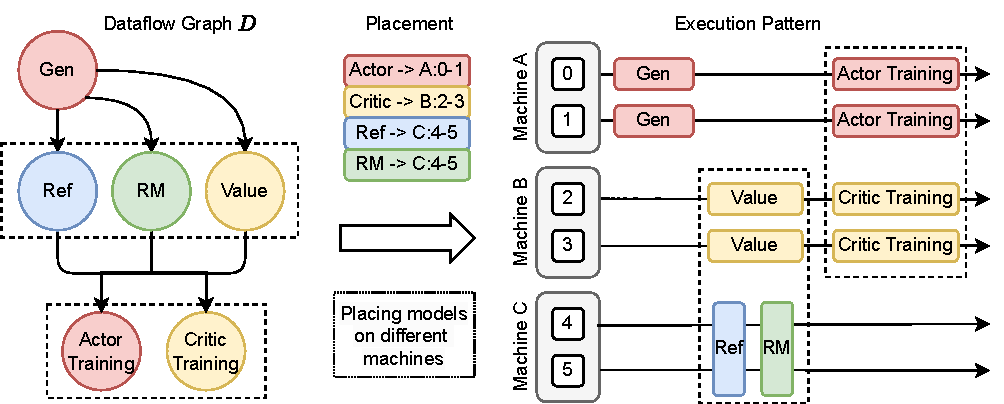
\includegraphics[width=\linewidth]{figs/fig_placement.pdf}
    \vspace{-5mm}
    \caption{Dataflow execution given a model placement plan. Blocks with numbers represent GPUs. In dashed boxes, the models are placed on different sets of devices and can be concurrently computed. Reference model (blue) and reward model (green) are colocated on the same set of GPUs and executed sequentially.}
    \vspace{-3mm}
    \label{fig:placement}
\end{figure}

\begin{table*}[t]
    \centering   
    \caption{Comparison of RLHF frameworks. Figures illustrate execution of one PPO iteration. Numbers 1-6 %
    represent response generation, reward model inference, reference model inference, critic inference, actor training, and critic training, respectively. %
    }
    \vspace{-3mm}
    \resizebox{\linewidth}{!}{%
    
    \begin{tabular}{c|c|c|c|c}
        \toprule
        RLHF system& DeepSpeed-Chat & OpenRLHF & NeMo-Aligner  &\textbf{HybridFlow} \\
        \midrule
        \makecell{Parallelism\\} & \makecell{Training: ZeRO \\ Generation:TP} & \makecell{Training: ZeRO \\ Generation:TP}  & \makecell{3D Parallelism for both\\ training and generation} & 
        \makecell{\textbf{Training: 3D, ZeRO, FSDP} \\ \textbf{Generation: 3D Parallelism}} 
        \\
        \midrule
        \makecell{Actor weights \\ in training \& generation} & \makecell{Model resharding\\ from ZeRO to TP} & \makecell{Using two copies of actor \\ weights for the two stages}  & \makecell{Using identical model partition \\ in two stages (shared weights)} &\makecell{\textbf{Zero-redundancy} \\ \textbf{model resharding} }\\
        \midrule
        \makecell{Model\\Placement} & \makecell{Colocate all models \\on the same set of devices} & \makecell{Each model placed \\on separate devices} & \makecell{Actor/Ref colocated on some GPUs\\Critic/RM colocated on other GPUs} &\textbf{\makecell{Support various \\ model placement}} \\
        \midrule
        \makecell{Execution\\Pattern\\
        \begin{minipage}{2cm}
            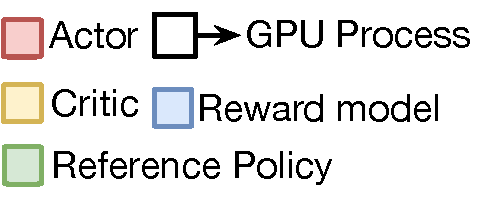
\includegraphics[width=\linewidth]{figs/fig_table_caption.pdf}
        \end{minipage}}
        &
        \begin{minipage}{2.5cm}
            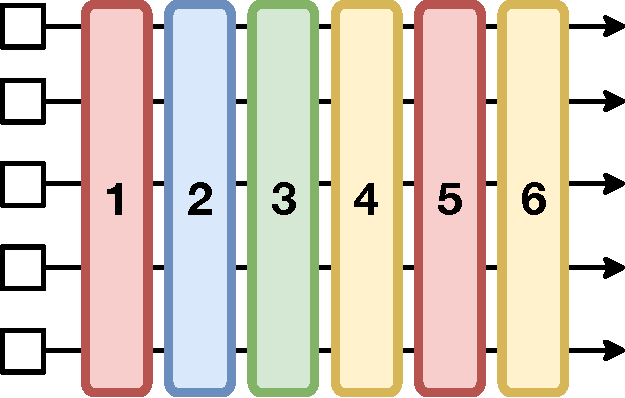
\includegraphics[width=\linewidth]{figs/fig_dschat.pdf}
        \end{minipage}
        &
        \begin{minipage}{2.3cm}
            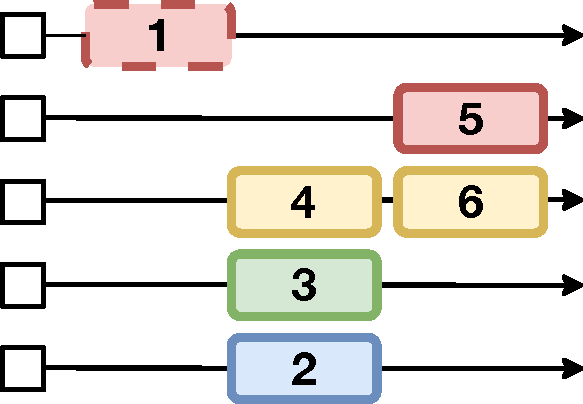
\includegraphics[width=\linewidth]{figs/fig_openrlhf.pdf}
        \end{minipage}
        &
        \begin{minipage}{2.3cm}
            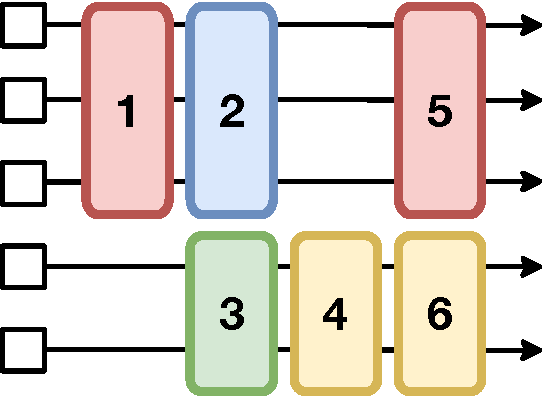
\includegraphics[width=\linewidth]{figs/fig_nemoaligner.pdf}
        \end{minipage}
        &
        \textbf{\makecell{Support various \\execution patterns}}
        \\
        \bottomrule
    \end{tabular}%
    }
    \label{tab:table_with_images}
    \vspace{-3mm}
\end{table*}


\noindent\textbf{Diverse model placement requirements.}
Strategic device placement of models in the RLHF dataflow is necessary, %
according to computation workloads and data dependencies of the models. Figure~\ref{fig:placement} gives an example model placement plan and the corresponding RLHF execution flow. %
Models placed on different sets of devices can be executed in parallel if no data dependencies exist. Models placed on the same set of GPUs, referred to as {\em colocated models}, share the GPU memory and are executed sequentially in a time-sharing manner, as out-of-memory (OOM) error may easily happen if colocated LLMs execute concurrently.  

We observe a compromise: placing models on different devices permits parallel processing but may inevitably lead to some GPU idle time, given staged model execution in RLHF.
In Figure~\ref{fig:placement}, actor and critic are placed separately, performing training in parallel, but incurring 1/3 of their GPU time being idle, during other RLHF stages. Supporting various placement strategies and maximizing device utilization %
are crucial for optimizing RLHF performance at any model size and cluster scale. 







    
    


    



    


\vspace{-1mm}
\subsection{Limitations of existing RLHF systems}
\vspace{-1mm}
\noindent\textbf{Inflexible support for various RLHF dataflow graphs.}
Existing RLHF systems %
adopt the multi-controller paradigm for dataflow implementation~\cite{yao2023deepspeedchat, hu23openrlhf, NeMoAligner, xiao2023adaptive}. %
{To implement various RLHF algorithms,}
a user must navigate and manage code %
that mixes collective communication, model computation (potentially using various distributed training/serving frameworks), and point-to-point data transfer. %
This %
code structure lacks %
modularity/function encapsulation, making the RLHF systems tightly coupled with specific LLM training and serving frameworks.
Consequently, a user needs to implement and optimize different RLHF dataflows case-by-case~\cite{liang2021rllib}, hindering code reuse and increasing the risk of making mistakes. Existing RLHF frameworks only support the PPO algorithm.
In addition, limited parallel strategies are supported due to implementation complexity. For example, to incorporate 3D parallelism for LLM training and generation
in DeepSpeed-Chat~\cite{yao2023deepspeedchat}, one may have to re-implement the whole system due to the mixed code structure.


\noindent\textbf{Inefficient RLHF execution.} %
Table~\ref{tab:table_with_images} summarizes parallelism strategies, model placement, and execution patterns adopted by the existing RLHF systems. %
DeepSpeed-Chat~\cite{yao2023deepspeedchat} and OpenRLHF~\cite{hu23openrlhf} adopt ZeRO-3 for actor training and TP for actor generation.
OpenRLHF uses different copies of the actor model on different devices for training and generation,
incurring redundant memory usage and frequent weight synchronization among devices.
DeepSpeed-Chat maintains the same copy of actor model on the same set of devices for training and generation, %
and reshards model weights between training and generation (due to different parallelisms used in the two stages), %
which may still incur substantial {memory and communication} overhead 
for large models (detailed in \textsection\ref{sec:hybrid_comm_mem}). 
NeMo-Aligner~\cite{NeMoAligner} uses the same 3D parallelism configurations in actor training and generation, %
experiencing low generation throughput  (\textsection\ref{sec:exp_benefit_hybrid_engine}).

Existing RLHF frameworks are limited to one model placement plan and hence one RLHF execution pattern, as shown in Table~\ref{tab:table_with_images}. Implementing a different placement is difficult, requiring changing the inner logic of 
{model initialization and inter-node data transfer as highlighted in blue in Figure~\ref{fig:program_model_compare}.}
OpenRLHF and NeMo-Aligner allow concurrent model computation in the preparation and learning stages; in the generation stage, models except the actor are idle, wasting the GPUs they occupy. 
DeepSpeed-Chat %
colocates all models on the same set of devices, 
and each device runs each model sequentially according to the RLHF dataflow. With unbalanced workloads among the models, such a placement can be inefficient in resource utilization
(evaluated in \textsection\ref{sec:exp_placement}).












\vspace{-2mm}
\subsection{Design Considerations}
To tackle limitations of existing systems,
the key question is -
\textbf{How to design a flexible and efficient programming model to implement RLHF dataflow?}
A single-controller design is particularly advantageous at the inter-node level due to its flexibility in coordinating data transfer, execution order, and resource virtualization among distributed computation of different models~\cite{barham2022pathways, moritz2018ray}. 
The RLHF dataflow graph  %
typically consists of only a few nodes. %
Dispatching control messages to different nodes from the single-controller %
incurs negligible overhead as compared to distributed computation required for nodes (models) in the dataflow.
The multi-controller paradigm, known for its low latency in dispatching operators to accelerators~\cite{darema2001spmd}, can be leveraged in distributed computation of each model.
With these insights, we propose a hierarchical hybrid programming model for RLHF dataflow implementation.
Our key design principle is to combine single-controller and multi-controller paradigms in a hybrid manner. %
This design ensures flexible expression and efficient execution of RLHF dataflow, maintaining low control overhead at both inter-node and intra-node levels.
As shown in Figure~\ref{fig:program_model_compare}(b), this paradigm decouples intra-node distributed computation and inter-node data transfer, allowing {each model}
to focus solely on local computation without managing inter-node communication. %



